% Provenance (never printed): see sources/outline_sources.md (Year 3:
% critical-taper theory; fold-and-thrust belts; exhumation and
% thermochronology). Brief: sources/book5/BRIEFS.md, ch. 10. Curves from
% figdata/bachelor-3/fault_bend.py, critical_taper.py and age_elevation.py.
% Exercise and problem values in the Book 5 scratch calculator calc/ch10.py.
\chapter{逆冲带与造山楔}\label{ch:b3:orogenic-wedges}

用推土机把湿沙或积雪向前推，物质便会在铲刀前堆成
一个楔形体。它不断变形，直到其表面达到某一坡度；
此后它便整体向前滑动，并保持相同形态而不断生长，在其前端吸纳新的物质。
造山带的外缘，从台湾到阿尔卑斯山麓，都以相同方式运动：
它们是从板块上刮下、推覆于软弱底层之上的岩石楔形体，
其表面坡度与底面倾角，
说明底面有多软弱，以及其中流体的压力有多高。本章建立
逆冲带的几何形态、
楔体的力学规律，以及
测定岩石上升至地表快慢的计时方法。
% ledger: dsd83:taper

\begin{recall}
逆冲断层、指向性与褶皱几何，见本科一年级分册中
关于断层、褶皱与织构的一章；库仑判据、拜尔利定律、有效应力，以及孔隙压力比 $\lambda = P/\sigma_v$，
见其中关于应力、应变与流变学的一章；
封闭温度与冷却年龄，见
其中关于放射性测年方法的一章。滑脱面、褶皱–逆冲带、薄皮与厚皮构造，
以及平衡剖面，见本科二年级分册中
关于造山带解剖的一章；折返及其速率，见
其中关于 P--T--t 轨迹的一章。
扭折作图法，以及\omterm{def:b3:orogenic-wedges:thrust-folds}{滑脱褶皱}之上的超出面积 $A = Sh$，
参见\cref{ch:b3:structural-analysis}；\omterm{def:b3:lithosphere-thermal-models:peclet}{热佩克莱数}见
\cref{ch:b3:lithosphere-thermal-models}。
\end{recall}

\section{逆冲断层的几何形态}\label{sec:b3:orogenic-wedges:geometry}

逆冲断层并非沿单一平面切穿层状岩系。
它沿软弱层延伸很远，软弱层可以是页岩或蒸发岩，
然后陡直地穿过上方的坚硬层，爬升至下一个软弱层。它
所勾勒的阶梯状轮廓控制着上盘的褶皱。

\begin{definition}[断坡、断坪、双重构造与无序逆冲断层]\label{def:b3:orogenic-wedges:thrust-geometry}
称\emph{断坪}\index{断坪}为沿层理近似平行延伸的逆冲断层段，通常位于
软弱层中；\emph{断坡}\index{断坡}为切过层理的断层段，
断坡的典型倾角为 20 至 \ang{30}，连接下方断坪与上方断坪。
\emph{双重构造}\index{双重构造}是由断层界定的构造岩片的叠置体，
这些岩片夹于下方的底板逆冲断层与上方的顶板逆冲断层之间，
每一岩片都被连接两者的断坡所切断。逆冲断层通常依次形成，
新生断层位于前一断层的下盘，并更靠近前陆；
\emph{无序逆冲断层}\index{无序逆冲断层}是
在活动前缘之后再次形成或滑动的断层，
它切割了较老的逆冲断层。
\end{definition}

上盘越过断层弯曲处时，为保持与断层接触必须褶皱：
在进入\omterm{def:b3:orogenic-wedges:thrust-geometry}{断坡}处形成向斜，
在离开\omterm{def:b3:orogenic-wedges:thrust-geometry}{断坡}处形成背斜。

\begin{definition}[断层转折褶皱、断层传播褶皱与滑脱褶皱]\label{def:b3:orogenic-wedges:thrust-folds}
\emph{断层转折褶皱}\index{断层转折褶皱}是逆冲断层上盘的一种褶皱，
由逆冲断层滑过断层弯曲时产生，该弯曲即
两\omterm{def:b3:orogenic-wedges:thrust-geometry}{断坪}之间的\omterm{def:b3:orogenic-wedges:thrust-geometry}{断坡}。\emph{断层传播褶皱}\index{断层传播褶皱}
生长于仍在向上扩展的逆冲断层尖端之上，
断层不再承载的缩短量由其尖端前方的褶皱吸收，
形成陡立或倒转的前翼。\emph{滑脱褶皱}\index{滑脱褶皱}生长于
无\omterm{def:b3:orogenic-wedges:thrust-geometry}{断坡}的\omterm{def:b3:orogenic-wedges:thrust-geometry}{断坪}之上，缩短量由褶皱及软弱层吸收，
该软弱层为盐或页岩，流入
褶皱的核部。
\end{definition}

下图构造了一个\omterm{def:b3:orogenic-wedges:thrust-folds}{断层转折褶皱}。此处上盘平行于其下方的断层段运动，
并沿轴面发生褶皱，这些轴面平分各个弯曲，
这是称为断层平行流动的运动学模型；经典模型
假定岩层厚度与长度不变，得到同样的平顶背斜，
但前翼更陡，代价是作图过程更长
（在本阶段不加证明地承认）。两种模型均受面积守恒约束。

\begin{omfigure}
\begin{tikzpicture}
\begin{groupplot}[group style={group size=1 by 2, vertical sep=0.9cm},
  width=0.92\linewidth, axis equal image,
  xmin=0, xmax=12, ymin=-0.6, axis lines=none, clip=true,
  title style={font=\small, at={(0.0,1.0)}, anchor=south west}]
% (a) before slip
\nextgroupplot[title={(a) 滑动前}, ymax=1.75]
\fill[omLithSand!70] (axis cs:0,0) rectangle (axis cs:12,1.6);
\fill[gray!25] (axis cs:0,-0.6) rectangle (axis cs:12,0);
\draw[black!70] (axis cs:0,0.25) -- (axis cs:12,0.25);
\draw[black!70] (axis cs:0,0.5) -- (axis cs:12,0.5);
\draw[black!70] (axis cs:0,0.75) -- (axis cs:12,0.75);
\draw[black!70] (axis cs:0,1.0) -- (axis cs:12,1.0);
\draw[black!70] (axis cs:0,1.3) -- (axis cs:12,1.3);
\draw[black!70] (axis cs:0,1.6) -- (axis cs:12,1.6);
\draw[black!70] (axis cs:0,-0.3) -- (axis cs:12,-0.3);
\addplot[very thick, red!70!black] table[x=x, y=y] {figdata/out/bachelor-3-fault_bend-fault.dat};
\node[font=\scriptsize, fill=omLithSand!70, inner sep=1pt] at (axis cs:2,0.125) {下断坪};
\node[font=\scriptsize, fill=omLithSand!70, inner sep=1pt, rotate=30] at (axis cs:4.55,0.62) {断坡};
\node[font=\scriptsize, fill=omLithSand!70, inner sep=1pt] at (axis cs:9,0.875) {上断坪};
% (b) after a slip of 2.5 units
\nextgroupplot[title={(b) 滑动后：断层转折褶皱}, ymax=2.75]
\fill[gray!25] (axis cs:0,-0.6) rectangle (axis cs:12,0) -- cycle;
\addplot[name path=fault, draw=none] table[x=x, y=y] {figdata/out/bachelor-3-fault_bend-fault.dat};
\addplot[name path=top, draw=none] table[x=x, y=y] {figdata/out/bachelor-3-fault_bend-bed6.dat};
\addplot[name path=base, draw=none] coordinates {(0,-0.6) (12,-0.6)};
\addplot[omLithSand!70] fill between[of=fault and top];
\addplot[gray!25] fill between[of=base and fault];
\addplot[black!70] table[x=x, y=y] {figdata/out/bachelor-3-fault_bend-bed1.dat};
\addplot[black!70] table[x=x, y=y] {figdata/out/bachelor-3-fault_bend-bed2.dat};
\addplot[black!70] table[x=x, y=y] {figdata/out/bachelor-3-fault_bend-bed3.dat};
\addplot[black!70] table[x=x, y=y] {figdata/out/bachelor-3-fault_bend-bed4.dat};
\addplot[black!70] table[x=x, y=y] {figdata/out/bachelor-3-fault_bend-bed5.dat};
\addplot[black!70] table[x=x, y=y] {figdata/out/bachelor-3-fault_bend-bed6.dat};
\draw[black!70] (axis cs:4.4330,0.25) -- (axis cs:12,0.25);
\draw[black!70] (axis cs:4.8660,0.5) -- (axis cs:12,0.5);
\draw[black!70] (axis cs:5.2990,0.75) -- (axis cs:12,0.75);
\draw[black!70] (axis cs:0,-0.3) -- (axis cs:12,-0.3);
\addplot[very thick, red!70!black] table[x=x, y=y] {figdata/out/bachelor-3-fault_bend-fault.dat};
\draw[densely dashed, black!60] (axis cs:0,1.6) -- (axis cs:12,1.6);
\node[font=\scriptsize, anchor=south] at (axis cs:2.2,1.65) {区域地表};
\node[font=\scriptsize, anchor=west] at (axis cs:8.6,2.25) {超出面积 $A = Sr$};
\draw[black!70] (axis cs:8.6,2.25) -- (axis cs:6.6,2.0);
\node[font=\scriptsize, fill=gray!25, inner sep=1pt] at (axis cs:10.6,0.625) {下盘};
\end{groupplot}
\end{tikzpicture}

\par\smallskip{\small (a) 逆冲断层，具有下部\omterm{def:b3:orogenic-wedges:thrust-geometry}{断坪}、倾角为
\ang{30} 的\omterm{def:b3:orogenic-wedges:thrust-geometry}{断坡}及上部\omterm{def:b3:orogenic-wedges:thrust-geometry}{断坪}，滑动前（示意图，竖直与水平比例尺相等）。
(b) 同一断层在滑动量为\omterm{def:b3:orogenic-wedges:thrust-geometry}{断坡}高度的 2.5 倍之后的情形，由平行于断层的流动计算得到：
\omterm{def:b3:orogenic-wedges:thrust-geometry}{断坡}底部的向斜、与\omterm{def:b3:orogenic-wedges:thrust-geometry}{断坡}平行的后翼、
被\omterm{def:b3:orogenic-wedges:thrust-geometry}{断坡}高度 $r$ 抬升的平坦顶部、前翼，
以及上部\omterm{def:b3:orogenic-wedges:thrust-geometry}{断坪}以上每一岩层相对区域水平面的
超出面积 $Sr$。}\label{fig:b3:orogenic-wedges:thrusts}
\end{omfigure}


\begin{proposition}[断层转折褶皱的超出面积]\label{prop:b3:orogenic-wedges:fault-bend-area}
设逆冲断层使其上盘沿高度为 $r$ 的\omterm{def:b3:orogenic-wedges:thrust-geometry}{断坡}，由下部\omterm{def:b3:orogenic-wedges:thrust-geometry}{断坪}
抬升至上部\omterm{def:b3:orogenic-wedges:thrust-geometry}{断坪}，下部\omterm{def:b3:orogenic-wedges:thrust-geometry}{断坪}上的滑动量为 $S$。对上盘中位于
上部\omterm{def:b3:orogenic-wedges:thrust-geometry}{断坪}之上的任一岩层，被弯曲岩层与其原始水平面所围的面积为
$A = Sr$，且对每一这样的岩层均相同。
\end{proposition}

\begin{proof}
岩石既不会产生也不会消失，其体积保持不变。取一与滑动方向平行的
剖面，以远离\omterm{def:b3:orogenic-wedges:thrust-geometry}{断坡}后方和
前方的两条竖直线为边界。穿过后方竖直线，下部\omterm{def:b3:orogenic-wedges:thrust-geometry}{断坪}与
其上高度为 $y_0$ 的岩层之间的上盘已向内移动 $S$，面积
$Sy_0$ 已进入。穿过前方竖直线，上部\omterm{def:b3:orogenic-wedges:thrust-geometry}{断坪}与
同一岩层之间、厚度为 $y_0 - r$ 的岩石，已因上部\omterm{def:b3:orogenic-wedges:thrust-geometry}{断坪}上的滑动向外
移出；若岩石保持面积不变，上部\omterm{def:b3:orogenic-wedges:thrust-geometry}{断坪}上的滑动量同样为 $S$，面积 $S(y_0 - r)$
已移出。二者之差 $Sr$ 留存于两线之间，并将
该岩层抬升至其原始水平面之上。
\end{proof}

\omterm{def:b3:orogenic-wedges:thrust-folds}{断层转折褶皱}的超出面积度量的是滑动量乘以
\omterm{def:b3:orogenic-wedges:thrust-geometry}{断坡}高度，而不是滑动量乘以滑脱面的深度；后者正是
\omterm{def:b3:orogenic-wedges:thrust-folds}{滑脱褶皱}的情形（见\cref{ch:b3:structural-analysis}）。两类褶皱
在将面积换算为缩短量之前，必须加以区分。


\omterm{def:b3:orogenic-wedges:thrust-geometry}{双重构造}（见下图）的形成方式是：逆冲断层不再沿同一\omterm{def:b3:orogenic-wedges:thrust-geometry}{断坡}继续
搬运其上盘，而是放弃该\omterm{def:b3:orogenic-wedges:thrust-geometry}{断坡}，并在下盘中切出一条新\omterm{def:b3:orogenic-wedges:thrust-geometry}{断坡}，
位于旧\omterm{def:b3:orogenic-wedges:thrust-geometry}{断坡}之前。旧\omterm{def:b3:orogenic-wedges:thrust-geometry}{断坡}与新\omterm{def:b3:orogenic-wedges:thrust-geometry}{断坡}之间的部分成为一个岩片，
沿新\omterm{def:b3:orogenic-wedges:thrust-geometry}{断坡}抬升，并叠置于顶板逆冲断层之下；下一条\omterm{def:b3:orogenic-wedges:thrust-geometry}{断坡}
又在前方形成。每一岩片从其原始长度缩短至沿底板的
现有长度，\omterm{def:b3:orogenic-wedges:thrust-geometry}{双重构造}的缩短量为各岩片缩短量之和。
\omterm{def:b3:orogenic-wedges:thrust-geometry}{无序逆冲断层}会打破这一顺序：它们形成于当前缘后方的楔体必须增厚时，
这一情形由下一节的
力学所预言。

\begin{omfigure}
\begin{tikzpicture}
\begin{axis}[width=0.92\linewidth, axis equal image, xmin=0, xmax=12, ymin=-0.6, ymax=1.95,
  axis lines=none, clip=true]
\fill[gray!25] (axis cs:0,-0.6) rectangle (axis cs:12,0);
\fill[omLithSand!70] (axis cs:0,0) -- (axis cs:1.0,0) -- (axis cs:2.35,1.15) -- (axis cs:12,1.15) -- (axis cs:12,1.85) -- (axis cs:2.35,1.85) -- (axis cs:1.0,0.7) -- (axis cs:0,0.7) -- cycle;
\draw[black!70] (axis cs:0,0.35) -- (axis cs:1.0,0.35) -- (axis cs:2.35,1.5) -- (axis cs:12,1.5);
\draw[black!70] (axis cs:0,0.7) -- (axis cs:1.0,0.7) -- (axis cs:2.35,1.85) -- (axis cs:12,1.85);
\fill[omLithShale!60] (axis cs:8.2,0) -- (axis cs:12,0) -- (axis cs:12,1.15) -- (axis cs:9.55,1.15) -- cycle;
\draw[black!70] (axis cs:8.646,0.38) -- (axis cs:12,0.38);
\draw[black!70] (axis cs:9.104,0.77) -- (axis cs:12,0.77);
\fill[omLithLime] (axis cs:1.0,0) -- (axis cs:2.80,0) -- (axis cs:4.15,1.15) -- (axis cs:2.35,1.15) -- cycle;
\draw[black!70] (axis cs:1.45,0) -- (axis cs:2.80,1.15);
\draw[black!70] (axis cs:1.90,0) -- (axis cs:3.25,1.15);
\draw[black!70] (axis cs:2.35,0) -- (axis cs:3.70,1.15);
\fill[omLithShale] (axis cs:2.8,0) -- (axis cs:4.60,0) -- (axis cs:5.95,1.15) -- (axis cs:4.15,1.15) -- cycle;
\draw[black!70] (axis cs:3.25,0) -- (axis cs:4.60,1.15);
\draw[black!70] (axis cs:3.70,0) -- (axis cs:5.05,1.15);
\draw[black!70] (axis cs:4.15,0) -- (axis cs:5.50,1.15);
\fill[omLithLime] (axis cs:4.6,0) -- (axis cs:6.40,0) -- (axis cs:7.75,1.15) -- (axis cs:5.95,1.15) -- cycle;
\draw[black!70] (axis cs:5.05,0) -- (axis cs:6.40,1.15);
\draw[black!70] (axis cs:5.50,0) -- (axis cs:6.85,1.15);
\draw[black!70] (axis cs:5.95,0) -- (axis cs:7.30,1.15);
\fill[omLithShale] (axis cs:6.4,0) -- (axis cs:8.20,0) -- (axis cs:9.55,1.15) -- (axis cs:7.75,1.15) -- cycle;
\draw[black!70] (axis cs:6.85,0) -- (axis cs:8.20,1.15);
\draw[black!70] (axis cs:7.30,0) -- (axis cs:8.65,1.15);
\draw[black!70] (axis cs:7.75,0) -- (axis cs:9.10,1.15);
\draw[thick, red!70!black] (axis cs:1.0,0) -- (axis cs:2.35,1.15);
\draw[thick, red!70!black] (axis cs:2.8,0) -- (axis cs:4.15,1.15);
\draw[thick, red!70!black] (axis cs:4.6,0) -- (axis cs:5.95,1.15);
\draw[thick, red!70!black] (axis cs:6.4,0) -- (axis cs:7.75,1.15);
\draw[thick, red!70!black] (axis cs:8.2,0) -- (axis cs:9.55,1.15);
\draw[very thick, red!70!black] (axis cs:0,0) -- (axis cs:12,0);
\draw[very thick, red!70!black] (axis cs:2.35,1.15) -- (axis cs:12,1.15);
\node[font=\scriptsize, anchor=north west] at (axis cs:0.1,-0.04) {底板逆冲断层};
\node[font=\scriptsize, anchor=south west] at (axis cs:7.0,1.17) {顶板逆冲断层};
\node[font=\scriptsize, anchor=north] at (axis cs:5.6,-0.12) {岩片};
\draw[black!70] (axis cs:5.6,-0.15) -- (axis cs:5.5,0.45);
\draw[->, thick] (axis cs:0.15,0.52) -- (axis cs:0.95,0.52);
\end{axis}
\end{tikzpicture}

\par\smallskip{\small \omterm{def:b3:orogenic-wedges:thrust-geometry}{双重构造}（示意图）：四个岩片（蓝色和绿色）由
底板与顶板逆冲断层之间的\omterm{def:b3:orogenic-wedges:thrust-geometry}{断坡}切割而成，其前方尚未被切割的下盘，
箭头指示搬运方向；顶板之上的盖层
在岩片叠置体上方发生褶皱。}\label{fig:b3:orogenic-wedges:duplex}
\end{omfigure}


\section{临界楔角}\label{sec:b3:orogenic-wedges:taper}

在剖面上，褶皱–逆冲带是一个楔体：其前缘较薄，在此处
滑脱面到达地表，并向后陆方向逐渐增厚。
其上表面以角度 $\alpha$ 向前陆方向倾斜；其
底面即滑脱面，以角度 $\beta$ 向后陆方向倾斜。楔体的
楔角即两者之间的夹角，$\alpha + \beta$。

\begin{definition}[临界楔角]\label{def:b3:orogenic-wedges:critical-taper}
称被后方推动、位于某一底面之上的楔体的\emph{临界楔角}\index{临界楔角}，
即在水平挤压下，楔体内部及沿其底面处处濒临
破坏的楔角。
处于临界楔角的楔体沿其底面滑动而内部不发生变形；
楔角小于临界楔角（次临界）的楔体会变形并增厚，直至达到该楔角；
楔角大于临界楔角（超临界）的楔体则滑动而不发生变形。
\end{definition}
% ledger: dsd83:taper

\begin{omfigure}
\begin{tikzpicture}[>=stealth, x=1cm, y=1cm]
\fill[omLithSand!70] (0,0) -- (10,-1.05) -- (10,1.4) -- cycle;
\fill[gray!25] (0,0) -- (10,-1.05) -- (10,-1.6) -- (-0.8,-1.6) -- (-0.8,0) -- cycle;
\draw[thick] (-0.8,0) -- (0,0) -- (10,1.4);
\draw[very thick, red!70!black] (0,0) -- (10,-1.05);
\fill[gray!60] (10,-1.6) rectangle (10.6,1.9);
\node[font=\scriptsize, rotate=90] at (10.3,0.15) {挡板};
\draw[dashed] (0,0) -- (2.6,0);
\draw (2.2,0) arc[start angle=0, end angle=8, radius=2.2];
\node[font=\small] at (2.45,0.2) {$\alpha$};
\draw (2.2,0) arc[start angle=0, end angle=-6, radius=2.2];
\node[font=\small] at (2.45,-0.2) {$\beta$};
% slice
\draw[thick, omDef] (5.5,-0.5775) -- (5.5,0.77);
\draw[thick, omDef] (6.5,-0.6825) -- (6.5,0.91);
\draw[->, thick, omDef] (4.5,0.05) -- (5.45,0.05);
\node[font=\scriptsize, anchor=east] at (4.5,0.05) {$F(x)$};
\draw[<-, thick, omDef] (6.55,0.1) -- (7.6,0.1);
\node[font=\scriptsize, anchor=west] at (7.6,0.1) {$F(x + \mathrm dx)$};
\draw[->, thick, omProp] (6.0,-0.63) -- (6.75,-0.71);
\node[font=\scriptsize, anchor=north] at (6.4,-0.75) {$\tau_b$};
\draw[->, thick, omProp] (6.0,-0.63) -- (6.1,0.0);
\node[font=\scriptsize, anchor=east] at (6.02,-0.22) {$\sigma_n$};
\node[font=\scriptsize] at (6.0,1.2) {切片 $\mathrm dx$};
\draw[->, thick] (1.8,-1.25) -- (0.6,-1.25);
\node[font=\scriptsize, anchor=west] at (1.85,-1.25) {输运};
\node[font=\scriptsize, anchor=west] at (0.2,-0.42) {滑脱面};
\node[font=\scriptsize] at (8.9,-0.45) {楔体};
\draw[->] (0.1,0.5) -- (0.4,0.5); \node[font=\scriptsize, anchor=east] at (0.1,0.5) {$x$};
\end{tikzpicture}

\par\smallskip{\small 楔体的地表坡度为 $\alpha$，搁置于
倾角为 $\beta$ 的滑脱面之上，并受后方推动；$x$ 自前缘
起朝向腹地方向量度。在竖直剖面上，来自后方的推力 $F(x + \mathrm dx)$
超出来自前方推力 $F(x)$ 的部分，由底面承担，
即其摩擦力 $\tau_b$ 与法向应力 $\sigma_n$ 的水平分量，
法向应力随向腹地倾斜的底面而朝腹地方向倾斜（示意图，
角度有所夸大）。}\label{fig:b3:orogenic-wedges:wedge}
\end{omfigure}

\begin{theorem}[临界楔方程]\label{thm:b3:orogenic-wedges:critical-taper}
考虑一个陆上楔体，密度 $\rho$ 均匀，由无内聚力的库仑材料构成，
其内摩擦系数 $\mu = \tan\phi$，孔隙压力比 $\lambda$，
楔体位于摩擦系数为 $\mu_b$、孔隙压力比为
$\lambda_b$ 的底面之上。若 $\alpha$ 与 $\beta$ 均较小，且 $\sigma_1$ 水平，
则\emph{临界楔方程}\index{临界楔方程}为
\[
  \alpha + \beta = \frac{\beta + \mu_b(1 - \lambda_b)}{1 + K(1 - \lambda)},
  \qquad K = \frac{2\sin\phi}{1 - \sin\phi},
\]
式中角度以弧度计。
\end{theorem}

\begin{proof}
设 $z$ 为地表以下的深度。坡度较小时，竖直应力
即上覆岩石的重量 $\sigma_{zz} = \rho g z$，孔隙压力为
$\lambda\rho g z$，故有效竖直应力为
$(1 - \lambda)\rho g z$。各处均处于破坏状态，且 $\sigma_1$ 水平，
对无内聚力材料，库仑判据给出有效主应力之比
$\sigma'_1/\sigma'_3 = (1 + \sin\phi)/(1 -
\sin\phi) = 1 + K$，于是总水平应力为
\[
  \sigma_{xx} = (1 + K)(1 - \lambda)\rho g z + \lambda\rho g z
  = \bigl(1 + K(1 - \lambda)\bigr)\rho g z .
\]
距前缘 $x$ 处，楔体厚度为 $H = (\alpha +
\beta)x$，则单位长度造山带在竖直截面上所受的水平力
为 $F = \int_0^H \sigma_{xx}\,\mathrm dz = \bigl(1 + K(1 -
\lambda)\bigr)\rho g H^2/2$。位于 $x$ 与 $x + \mathrm dx$ 之间的切片（见上图），
地表不承受应力，来自后方的推力超出
来自前方推力的部分为 $(\mathrm dF/\mathrm dx)\,\mathrm dx$。
底面以两种方式阻挡该切片：一是摩擦力 $\mu_b(1 -
\lambda_b)\rho g H$（按单位长度计），二是其法向应力 $\rho g H$，它
垂直于向腹地倾斜 $\beta$ 的底面，故朝该方向倾斜 $\beta$，
由此得水平分量 $\beta\rho g H$。
切片的平衡要求
\[
  \bigl(1 + K(1 - \lambda)\bigr)\rho g H(\alpha + \beta)
  = \bigl(\beta + \mu_b(1 - \lambda_b)\bigr)\rho g H ,
\]
即所求方程。由于 $H$ 约去，处于破坏状态的楔体保持相同的
楔角随其增长而不变。
\end{proof}

该方程表明：第一，楔角由底面强度与楔体强度之比决定，
其中底面强度位于分子，楔体强度位于分母；
底面弱则楔体薄，底面强则楔体厚。
第二，底面倾斜越陡，地表坡度越小。第三，流体压力
会降低楔角：$\lambda = \lambda_b$ 增大时，底面强度的
损失比例大于楔体强度的损失比例。
下图给出西台湾拟合摩擦系数所对应的临界地表坡度。
各曲线下方的点为次临界楔体，会增厚；
曲线上方的点为超临界楔体，会发生滑动。
% ledger: dsd83:taper

\begin{omfigure}
\begin{tikzpicture}
\begin{axis}[omrecord, width=0.8\linewidth, height=0.5\linewidth,
  xlabel={底面倾角 $\beta$ (\unit{\degree})}, ylabel={地表坡度 $\alpha$ (\unit{\degree})},
  xmin=0, xmax=15, ymin=0, ymax=12, legend style={font=\scriptsize, at={(0.98,0.98)},
  anchor=north east, legend cell align=left}]
% computed in figdata/bachelor-3/critical_taper.py
\addplot[name path=t3, draw=none, forget plot] table[x=beta, y=t3] {figdata/out/bachelor-3-critical_taper-bands.dat};
\addplot[name path=t4, draw=none, forget plot] table[x=beta, y=t4] {figdata/out/bachelor-3-critical_taper-bands.dat};
\addplot[name path=t12, draw=none, forget plot] table[x=beta, y=t12] {figdata/out/bachelor-3-critical_taper-bands.dat};
\addplot[name path=t13, draw=none, forget plot] table[x=beta, y=t13] {figdata/out/bachelor-3-critical_taper-bands.dat};
\addplot[omLithEvap, area legend] fill between[of=t3 and t4];
\addlegendentry{楔角 3--\ang{4}（侏罗山）}
\addplot[omLithLime, area legend] fill between[of=t12 and t13];
\addlegendentry{楔角 12--\ang{13}}
\addplot[omDef, thick] table[x=beta, y=a040] {figdata/out/bachelor-3-critical_taper-curves.dat};
\addlegendentry{$\lambda = 0.4$}
\addplot[red!70!black, thick, densely dashed] table[x=beta, y=a070] {figdata/out/bachelor-3-critical_taper-curves.dat};
\addlegendentry{$\lambda = 0.7$}
\addplot[black, thick, densely dotted] table[x=beta, y=a090] {figdata/out/bachelor-3-critical_taper-curves.dat};
\addlegendentry{$\lambda = 0.9$}
\node[font=\scriptsize] at (axis cs:2.2,1.1) {次临界};
\node[font=\scriptsize] at (axis cs:1.6,8.6) {超临界};
\end{axis}
\end{tikzpicture}

\par\smallskip{\small 临界地表坡度随基底倾角的变化，取西台湾的
摩擦系数：内部 $\mu = 1.03$，基底 $\mu_b =
0.85$，并给出三种孔隙压力比 $\lambda = \lambda_b$；
“次临界”与“超临界”指 $\lambda = 0.7$ 的曲线。阴影带
为侏罗山逆冲楔的楔角 3 至 \ang{4}，以及其南侧
楔体的楔角 12 至 \ang{13}。}\label{fig:b3:orogenic-wedges:taper}
\end{omfigure}
% ledger: dsd83:taper, deville21:jura

楔体并非静止的物体：物质不断被加入其中，又不断被移出，
每一次变化都会使它偏离\omterm{def:b3:orogenic-wedges:critical-taper}{临界楔角}。

\begin{definition}[前缘增生，构造底垫]\label{def:b3:orogenic-wedges:accretion}
\emph{前缘增生}\index{前缘增生}是指楔体前端增加物质：滑脱面
向未变形的前陆沉积物中推进，并切出新的逆冲岩片。
\emph{构造底垫}\index{构造底垫}是指楔体底部、位于前缘之后的物质增加：
下盘的岩片被剥离，
并叠置于楔体之下，
常呈\omterm{def:b3:orogenic-wedges:thrust-geometry}{双重构造}。
\end{definition}

\omterm{def:b3:orogenic-wedges:accretion}{前缘增生}使楔体在楔角不变的情况下向前延长。\omterm{def:b3:orogenic-wedges:accretion}{构造底垫}
使其后部增厚、表面变陡，楔体在该处转为超临界，
并可能通过正断层伸展，直至楔角回落。侵蚀
的作用则相反：降低地表坡度，楔体转为次临界，
并因前缘后方的无序逆冲而增厚。
因此，侵蚀与变形相互耦合：快速被侵蚀的楔体需要使岩石更快地向上输送，
方能保持其楔角；被带到地表的岩石，
按下一节的意义而言较为年轻。

\begin{inthelab}[砂箱模型]
\begin{minipage}[t]{0.55\linewidth}\vspace{0pt}
在模拟砂箱模型中，将不同颜色的干砂层
平铺于长条形玻璃侧壁箱中。电动机缓慢推动一块竖直挡板压向砂层，
或从砂层下方抽出一块薄板；紧贴玻璃的照相机按固定间隔拍摄剖面。
砂层沿逆冲面破裂，生长出保持恒定楔角的楔体，
并形成与真实造山带相似的\omterm{def:b3:orogenic-wedges:thrust-geometry}{断坡}、\omterm{def:b3:orogenic-wedges:thrust-geometry}{双重构造}和反向逆冲。
砂层下方铺一层玻璃珠或硅胶泥，充当较弱的
滑脱面，此时楔体变得更薄、更宽。
戴维斯、苏佩与达伦发现，他们的干砂实验与
\omterm{def:b3:orogenic-wedges:critical-taper}{临界楔角}理论相吻合。将先后拍摄的照片加以配准，即可得到
模型内部的位移场。
\end{minipage}\hfill
\begin{minipage}[t]{0.42\linewidth}\vspace{0pt}
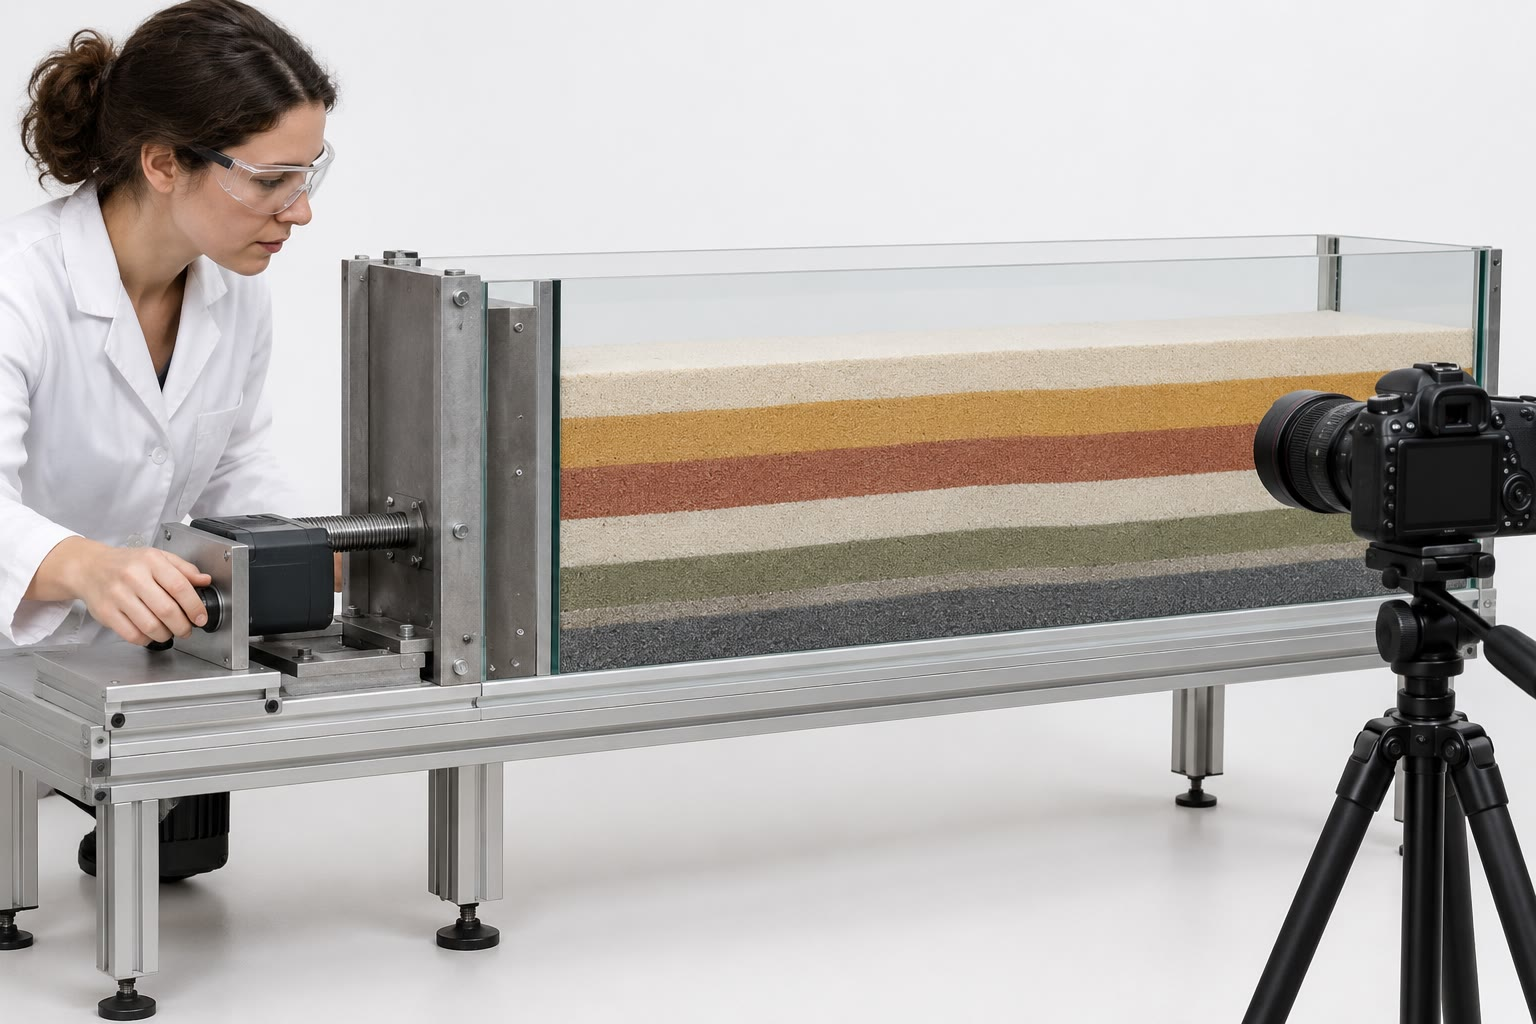
\includegraphics[width=\linewidth]{images/book5/ai/b3-sandbox-lab.jpg}

{\scriptsize 缩短前的砂箱模型：彩色砂层位于玻璃侧壁箱中，
左侧为电动机驱动的挡板，三脚架上安装有照相机
（AI 生成示意图）。}
\end{minipage}
\end{inthelab}
% ledger: dsd83:taper

\section{真实楔体}\label{sec:b3:orogenic-wedges:real}

在西台湾活动的褶皱–逆冲带中，地表坡度、
滑脱面倾角与孔隙压力均已知，其依据为地形、
地震剖面与钻井资料。戴维斯、苏佩与达伦利用这些资料求解
\omterm{thm:b3:orogenic-wedges:critical-taper}{临界楔方程}，以确定楔体强度，并得到内部 $\mu = 1.03$，
基底 $\mu_b = 0.85$，即拜尔利摩擦，而楔体
强度高于其自身断层，因为这些断层并非都处于易于滑动的取向。
利用这两个系数，他们将其他活动楔体（无论位于陆上还是海底）
所观测到的楔角换算为孔隙压力比，并发现它们都高于静水压力，
与钻探结果相符。他们还发现理论的适用范围：
楔体增厚至超过
约 \qty{15}{km} 时，楔角骤然下降，这一深度是常见地温线下石英质岩石
开始塑性变形的深度，此时底部不再服从摩擦定律。
% ledger: dsd83:taper

在西阿尔卑斯山前缘，侏罗山是一个楔角很窄的逆冲楔，
楔角仅为 3 至 \ang{4}。其滑脱面主要位于含岩盐的
三叠纪地层中，那里的流体并不超压：
仅盐的软弱性便足以解释狭窄的楔角。侏罗山以南，
三叠系不含岩盐，同一前缘的楔角为 12 至
\ang{13}，并有叠置的逆冲岩片，尽管该处实测的流体压力
较高。在中阿尔卑斯，对地表坡度进行\omterm{def:b3:orogenic-wedges:critical-taper}{临界楔角}分析，
得到基底强度 $\mu_b(1 - \lambda_b)$（含一小项内聚力）
低于 0.1，前缘附近的蒸发岩与页岩中甚至低至 0.05，
并向后陆方向增大，孔隙压力比高于 0.54。
楔体基底往往远弱于拜尔利定律所描述的强度，
其弱化既取决于岩性，也取决于流体。
% ledger: deville21:jura, vonhagke14:alps

\section{通过楔体的通量}\label{sec:b3:orogenic-wedges:flux}

处于\omterm{def:b3:orogenic-wedges:critical-taper}{临界楔角}的楔体通过增生而增长，形状保持不变：其长度
与高度同时增大。侵蚀移除地表岩石。当两者
达到平衡时，楔体的尺寸保持不变，岩石则从其中流过。

\begin{proposition}[稳态通量平衡]\label{prop:b3:orogenic-wedges:flux}
设宽度为 $W$ 的楔体沿输送方向，沿造山带单位长度接收
的增生通量 $F_a = v h$，其中 $v$ 为汇聚速率，
$h$ 为滑脱面之上输入岩层的厚度。它
损失的侵蚀通量为 $F_e = \bar e W$，其中 $\bar e$ 为
其表面的平均侵蚀速率。其截面面积以 $F_a -
F_e$ 的速率变化；稳态时，$\bar e = vh/W$。
\end{proposition}

\begin{proof}
单位时间内，长度为 $v$、厚度为 $h$ 的输入岩层越过
楔体前端进入楔体，并在其表面各点移除厚度 $e(x)$；
面积守恒，故剖面面积的变化为
$vh - \int_0^W e\,\mathrm dx = F_a - F_e$。稳态时
该变化为零。
\end{proof}

取 $v = \qty{10}{mm/\text{年}}$、$h = \qty{4}{km}$ 与 $W = \qty{60}{km}$，
稳态所需的侵蚀速率为 $\qty{0.67}{mm/\text{年}}$。按
本科二年级分册的意义，折返即移除某一岩石之上的岩石：
稳态时，岩石到达地表的速率等于侵蚀降低地表的速率，
楔体将它们从曾经较热的深处带上来。测定
折返速率需要一个从已知温度开始计时的时钟。

\section{热年代学}\label{sec:b3:orogenic-wedges:thermochronology}

\begin{definition}[热年代学，热年代计]\label{def:b3:orogenic-wedges:thermochronology}
\emph{热年代学}\index{热年代学}是利用放射性
冷却年龄确定岩石经过某一给定温度的时间，
从而重建其热历史。
\emph{热年代计}\index{热年代计}是一种矿物与一种定年方法的组合，
并给出其封闭温度，例如磷灰石
（U--Th）/He 法，或锆石的裂变径迹法。
\end{definition}

下表按封闭温度排列主要的\omterm{def:b3:orogenic-wedges:thermochronology}{热年代计}；
深度假设平均地表温度为 \qty{10}{\celsius}，
地温梯度均匀，为 \qty{30}{\celsius/km}。岩石在
折返过程中逐渐冷却，依次经过这些封闭温度，其年龄
从低温方法到高温方法逐渐增大。裂变径迹与氦扩散的物理机制
决定了这些温度，参见
\cref{ch:b3:advanced-geochronology}。
\begin{center}
\small
% ledger: sueoka19:closure
\begin{tabular}{lcc}
\hline
\omterm{def:b3:orogenic-wedges:thermochronology}{热年代计} & 封闭温度（\unit{\celsius}） & 深度（\unit{km}） \\
\hline
磷灰石（U--Th）/He & 50--80 & 1.3--2.3 \\
磷灰石裂变径迹 & 90--120 & 2.7--3.7 \\
锆石（U--Th）/He & 160--200 & 5.0--6.3 \\
锆石裂变径迹 & 约 280 & 9 \\
\textsuperscript{40}Ar/\textsuperscript{39}Ar（黑云母） & 350--400 & 11--13 \\
\textsuperscript{40}Ar/\textsuperscript{39}Ar（白云母） & 约 425 & 14 \\
U--Pb（锆石） & 高于 900 &——\\
\hline
\end{tabular}
\end{center}

这些深度只是初步估计，因为侵蚀会改变地温线。

\begin{proposition}[侵蚀作用下的稳态地温]\label{prop:b3:orogenic-wedges:geotherm}
设岩石以恒定速度 $v$ 通过厚度为 $L$ 的岩层上升，该岩层
地表（$z = 0$）温度保持为 $T_s$，底部温度为 $T_L$，
且无产热。稳态温度为
\[
  T(z) = T_s + (T_L - T_s)\,\frac{1 - e^{-\mathrm{Pe}\,z/L}}{1 - e^{-\mathrm{Pe}}},
  \qquad \mathrm{Pe} = \frac{vL}{\kappa},
\]
地表梯度为 $\mathrm{Pe}/(1 - e^{-\mathrm{Pe}})$ 倍
的传导梯度 $(T_L - T_s)/L$。
\end{proposition}

\begin{proof}
深度为 $z$ 的岩石质点向上运动，朝向较小的 $z$：其携带的
温度变化为 $\partial T/\partial t - v\,\partial
T/\partial z$，扩散方程变为 $\partial T/\partial t - v
T' = \kappa T''$。稳态时，$T'' = -(v/\kappa)T'$，故 $T' = C
e^{-vz/\kappa}$，$T = T_s + C(\kappa/v)(1 - e^{-vz/\kappa})$，并满足
$T(0) = T_s$。令 $T(L) = T_L$ 确定 $C$，即得公式。在 $z =
0$ 处，$T' = (T_L - T_s)(\mathrm{Pe}/L)/(1 - e^{-\mathrm{Pe}})$。
\end{proof}

当 $\mathrm{Pe} \ll 1$ 时，该因子趋于 1：传导占优，
地温线保持为直线。对于 $v = \qty{1}{mm/\text{年}}$、厚度 \qty{30}{km}，
$\kappa = \qty{e-6}{m^2/s}$，$\mathrm{Pe} = 0.95$，地表梯度
由 30 升至 \qty{46}{\celsius/km}：等温线向
地表聚集，每一种\omterm{def:b3:orogenic-wedges:thermochronology}{热年代计}的封闭深度都变浅。
% ledger: england:kelvin, earle:settings

\begin{definition}[年龄–高程关系]\label{def:b3:orogenic-wedges:age-elevation}
\emph{年龄–高程关系}\index{年龄–高程关系}是某一\omterm{def:b3:orogenic-wedges:thermochronology}{热年代计}的
冷却年龄图：取若干样品，其采样高程跨越一定范围，
通常沿陡坡或竖直剖面采集，
以冷却年龄对样品高程作图。
\end{definition}

\begin{proposition}[年龄–高程关系的斜率]\label{prop:b3:orogenic-wedges:age-elevation}
设岩石在稳态地形下以恒定速度 $v$ 竖直上升，
且封闭等温线位于高程 $e(x) = e_0 +
f\,h(x)$ 处，其中 $h(x)$ 为地表高程，$0 \le f < 1$。
在地表高程 $h$ 处采集的样品，其年龄为 $t = (h - e)/v$，
\omterm{def:b3:orogenic-wedges:age-elevation}{年龄–高程关系}为直线，其斜率为
\[
  \frac{\mathrm dh}{\mathrm dt} = \frac{v}{1 - f}.
\]
等温线水平时，$f = 0$，斜率即为折返速率。
\end{proposition}

\begin{proof}
地表 $x$ 处的岩石正是在其正下方穿过封闭等温线的，
即高程 $e(x)$ 处，此后上升了 $h - e$，速度为 $v$：
$t = (h - e_0 - fh)/v = ((1 - f)h - e_0)/v$。由此 $\mathrm dt/\mathrm dh =
(1 - f)/v$。
\end{proof}

\begin{omfigure}
\begin{tikzpicture}
\begin{groupplot}[group style={group size=2 by 1, horizontal sep=1.7cm},
  omrecord, width=0.47\linewidth, height=0.45\linewidth, title style={font=\small},
  legend style={font=\scriptsize, legend cell align=left}]
\nextgroupplot[title={(a) 年龄–高程}, xlabel={磷灰石（U--Th）/He 年龄（\unit{Ma}）},
  ylabel={高于平均值的高程（\unit{km}）}, xmode=log, xmin=0.1, xmax=10,
  log ticks with fixed point, xtick={0.1,0.2,0.5,1,2,5,10}, ymin=-1, ymax=1]
% computed in figdata/bachelor-3/age_elevation.py
\addplot[black, thick, densely dotted] table[x=a30, y=h] {figdata/out/bachelor-3-age_elevation-ages.dat};
\addplot[red!70!black, thick, densely dashed] table[x=a10, y=h] {figdata/out/bachelor-3-age_elevation-ages.dat};
\addplot[omDef, thick] table[x=a03, y=h] {figdata/out/bachelor-3-age_elevation-ages.dat};
\nextgroupplot[title={(b) 封闭等温线}, xlabel={距离（\unit{km}）},
  ylabel={高于平均值的高程（\unit{km}）}, xmin=0, xmax=40, ymin=-3.3, ymax=1.2,
  legend style={at={(0.5,0.03)}, anchor=south, legend columns=2}]
\addplot[black!70, very thick] table[x=x, y=h] {figdata/out/bachelor-3-age_elevation-iso.dat};
\addlegendentry{地表}
\addplot[black, thick, densely dotted] table[x=x, y=e30] {figdata/out/bachelor-3-age_elevation-iso.dat};
\addlegendentry{\qty{3}{mm/\text{年}}}
\addplot[red!70!black, thick, densely dashed] table[x=x, y=e10] {figdata/out/bachelor-3-age_elevation-iso.dat};
\addlegendentry{\qty{1}{mm/\text{年}}}
\addplot[omDef, thick] table[x=x, y=e03] {figdata/out/bachelor-3-age_elevation-iso.dat};
\addlegendentry{\qty{0.3}{mm/\text{年}}}
\end{groupplot}
\end{tikzpicture}

\par\smallskip{\small 在正弦起伏地形之下的稳态折返，
波长 \qty{20}{km}、振幅 \qty{1}{km}，三种速率，
线型与（b）的图例一致（一阶模型；岩层厚 \qty{30}{km}，地表温度 \qty{10}{\celsius}，
无侵蚀时的梯度 \qty{30}{\celsius/km}，$\kappa = \qty{e-6}{m^2/s}$，气温
直减率 \qty{6.5}{\celsius/km}，封闭温度 \qty{65}{\celsius}）。（a）年龄对
高程：斜率分别为 0.59、2.5 与 \qty{14}{mm/\text{年}}，而非 0.3、1 与 3。
（b）折返越快，\qty{65}{\celsius} 等温线
越紧密地跟随地形，因其上升得离地表更近。}\label{fig:b3:orogenic-wedges:age-elevation}
\end{omfigure}
% ledger: earle:settings, england:kelvin, ussa76:layers, sueoka19:closure

等温线在起伏地形之下并不水平：峰顶处的地表比谷底更冷，
温差由大气气温直减率决定，但远小于同一海拔地下岩石中的温差，
而浅层等温线
以较为缓和的方式跟随地形。对于正弦地形，
波长为 $\Lambda$、气温直减率为 $\Gamma$ 时，
稳态方程的一阶解给出
\[
  f = \frac{(G_0 - \Gamma)\,e^{-mz_c}}{G(z_c)},\qquad
  m = \frac{v}{2\kappa} + \sqrt{\Bigl(\frac{v}{2\kappa}\Bigr)^2 +
  \Bigl(\frac{2\pi}{\Lambda}\Bigr)^2},
\]
其中 $z_c$ 为封闭等温线位于平均地表以下的深度，
$G_0$ 为地表梯度，$G(z_c)$ 为 $z_c$ 处的梯度（在本阶段不加证明地承认；
脚本会对其进行检验）。扰动随深度衰减，其衰减距离
为 $1/m$，至多为 $\Lambda/2\pi$：低温\omterm{def:b3:orogenic-wedges:thermochronology}{热年代计}
它们在浅部封闭，对起伏地形最为敏感。上图给出了
磷灰石 (U--Th)/He 的此种效应。
% ledger: sueoka19:closure, ussa76:layers

年龄–高程剖面只有在封闭等温线于起伏地形之下为水平时，才能测得折返速率，
否则将以因子 $1/(1 - f)$ 高估折返速率，该因子在
波长为 \qty{20}{km} 起伏地形中的磷灰石 (U--Th)/He 体系下达到两倍或更大。
同一样品上多种\omterm{def:b3:orogenic-wedges:thermochronology}{热年代计}所得的年龄，以及起伏地形的热模型，
可用于对此进行校正。

\section{练习}

\begin{exercise}[$\star$]\label{exo:b3:orogenic-wedges:1}
求楔体破坏时的 $K$ 与比值 $\sigma'_1/\sigma'_3$，
楔体的 $\phi = \ang{30}$。
\end{exercise}

\begin{exercise}[$\star$]\label{exo:b3:orogenic-wedges:2}
干砂楔体（$\lambda = \lambda_b = 0$）内部 $\mu = 0.6$，
其底面 $\mu_b = 0.3$。求其临界地表坡度，分别为水平底面，
以及底面倾角为 \ang{3} 时的值。
\end{exercise}

\begin{exercise}[$\star$]\label{exo:b3:orogenic-wedges:3}
地表温度为 \qty{10}{\celsius}，梯度为 \qty{30}{\celsius/km}，
核对封闭温度表中磷灰石 (U--Th)/He、
磷灰石裂变径迹与锆石裂变径迹所对应的深度。哪一种
\omterm{def:b3:orogenic-wedges:thermochronology}{热年代计}最适合用于测定自 \qty{5}{km} 深处开始的折返？
\end{exercise}

\begin{exercise}[$\star$]\label{exo:b3:orogenic-wedges:4}
一段高 \qty{2}{km} 的\omterm{def:b3:orogenic-wedges:thrust-geometry}{断坡}，倾角为 \ang{30}。求其水平长度与
沿倾向的长度。上盘岩层越过整个\omterm{def:b3:orogenic-wedges:thrust-geometry}{断坡}后被抬升了多少，
以及多大的滑移量才能使最下层岩层的截断点
从\omterm{def:b3:orogenic-wedges:thrust-geometry}{断坡}底部到达上部\omterm{def:b3:orogenic-wedges:thrust-geometry}{断坪}？
\end{exercise}

\begin{exercise}[$\star\star$]\label{exo:b3:orogenic-wedges:5}
采用台湾系数，求底面
倾角为 \ang{6}、$\lambda = \lambda_b = 0.4$ 与 $0.9$ 时的临界地表坡度。流体压力的增大
对原处于\omterm{def:b3:orogenic-wedges:critical-taper}{临界楔角}的楔体会产生什么影响？
\end{exercise}

\begin{exercise}[$\star\star$]\label{exo:b3:orogenic-wedges:6}
一个\omterm{def:b3:orogenic-wedges:thrust-folds}{断层转折褶皱}位于高 \qty{1.5}{km} 的\omterm{def:b3:orogenic-wedges:thrust-geometry}{断坡}之上，上部\omterm{def:b3:orogenic-wedges:thrust-geometry}{断坪}之上的一层岩层
显示其超出面积为 \qty{6.0}{km^2}。求滑移量。一位同事
将同一褶皱解释为\omterm{def:b3:orogenic-wedges:thrust-folds}{滑脱褶皱}，该岩层位于
滑脱面之上 \qty{3.0}{km} 处。他会得到多大的缩短量？
\end{exercise}

\begin{exercise}[$\star\star$]\label{exo:b3:orogenic-wedges:7}
取汝拉楔体（楔角 \ang{3.5}）及其南侧楔体（楔角 \ang{12.5}）内部的 $\mu = 0.6$，
两者内部均取静水条件 $\lambda = 0.4$，
两者基底倾角均为 \ang{2}。计算各楔角所要求的基底强度 $\mu_b(1 -
\lambda_b)$ 为各楔角所需的值，并与静水压力下拜尔利的 $0.85$ 相比较。
该结果是否与汝拉之下
岩盐中的滑脱面相符？
\end{exercise}

\begin{exercise}[$\star\star$]\label{exo:b3:orogenic-wedges:8}
岩石以 \qty{1}{mm/\text{年}} 的速度穿过厚 \qty{30}{km} 的岩层上升，
自底部 \qty{910}{\celsius} 升至地表 \qty{10}{\celsius}，
并取 $\kappa = \qty{e-6}{m^2/s}$。求\omterm{def:b3:lithosphere-thermal-models:peclet}{热佩克莱数}、地表梯度，
以及 \qty{65}{\celsius} 等温线的深度。
并与无侵蚀时的深度进行比较。
\end{exercise}

\begin{exercise}[$\star\star$]\label{exo:b3:orogenic-wedges:9}
同一坡面上的两个样品，分别位于 1200 与 \qty{2000}{m} 处，磷灰石
(U--Th)/He 年龄分别为 3.4 与 \qty{4.6}{Ma}。求表观折返
速率。起伏地形的热模型给出 $f = 0.5$，真实速率是多少？
\end{exercise}

\begin{exercise}[$\star\star\star$]\label{exo:b3:orogenic-wedges:10}
证明：当 $\lambda = \lambda_b$ 时，临界地表坡度在
基底倾角 $\beta^* = \mu_b/K$ 处为零，该倾角与 $\lambda$ 无关。计算
台湾对应的数值。若基底倾角更陡，楔体会怎样？
\end{exercise}

\begin{exercise}[$\star\star\star$]\label{exo:b3:orogenic-wedges:11}
证明：当波长很长、折返很慢时，$f$ 趋于
$1 - \Gamma/G$，其中 $G$ 为均匀梯度；取 $G =
\qty{30}{\celsius/km}$，$\Gamma = \qty{6.5}{\celsius/km}$，求此时
\omterm{def:b3:orogenic-wedges:age-elevation}{年龄–高程关系}的斜率是多少？对于 $v = \qty{1}{mm/\text{年}}$，
并取练习~8 中的数值（$z_c = \qty{1.21}{km}$，$G_0 = \qty{46.5}{\celsius/km}$，
$G(z_c) = \qty{44.7}{\celsius/km}$），求波长为 5 与
\qty{20}{km} 时的 $f$。
\end{exercise}

\begin{exercise}[$\star\star\star$]\label{exo:b3:orogenic-wedges:12}
楔体以\omterm{def:b3:orogenic-wedges:critical-taper}{临界楔角} $\alpha + \beta$ 生长，仅依靠\omterm{def:b3:orogenic-wedges:accretion}{前缘增生}，
不计侵蚀，由通量 $F_a$ 供给。证明其宽度按
$W = \sqrt{2F_at/\tan(\alpha + \beta)}$ 增长。取 $F_a = \qty{40}{km^2/Ma}$，
楔角为 \ang{6}，求经过 \qty{2}{Ma} 后其宽度，
并求其达到 \qty{60}{km} 所需的时间？
\end{exercise}

\section{问题：凯斯特雷尔楔体的前缘}

\begin{problem}[{周末问题——虚构逆冲楔体的缩短、力学、
通量与折返}]
\label{pb:b3:orogenic-wedges:1}
% values: calc/ch10.py; critical_taper.py; age_elevation.py; fault_bend.py
凯斯特雷尔山脉是一虚构造山带的前缘，即一条陆上
褶皱–逆冲带，宽 \qty{60}{km}，以 \qty{10}{mm/\text{年}} 的速率向
前陆推进，前陆之上的沉积层厚 \qty{4.0}{km}，位于页岩
滑脱面之上。其前缘逆冲断层沿滑脱面延伸，该滑脱面位于地表以下 \qty{4.5}{km}，
随后爬上倾角为 \ang{25} 的\omterm{def:b3:orogenic-wedges:thrust-geometry}{断坡}，并沿上部\omterm{def:b3:orogenic-wedges:thrust-geometry}{断坪}
延伸，\omterm{def:b3:orogenic-wedges:thrust-geometry}{断坪}埋深 \qty{1.5}{km}。前缘处地表高出海平面 \qty{0.3}{km}，
滑脱面位于其下 \qty{4.0}{km}；距前缘 \qty{60}{km} 处，
地表高程为 \qty{2.4}{km}，滑脱面位于
海平面以下 \qty{8.2}{km}。参照台湾的情形，取 $\mu = 1.03$ 与 $\mu_b =
0.85$，岩石密度 \qty{2500}{kg/m^3}，水的密度 \qty{1000}{kg/m^3}，
$g = \qty{9.81}{m/s^2}$.

\medskip\noindent\textbf{第一部分——逆冲几何。}
\begin{enumerate}
  \item 求\omterm{def:b3:orogenic-wedges:thrust-geometry}{断坡}的高度、水平长度以及
        沿倾角方向的长度。
  \item 上盘中某一层穿过
        整个\omterm{def:b3:orogenic-wedges:thrust-geometry}{断坡}后被抬升了多少？
  \item \omterm{def:b3:orogenic-wedges:thrust-geometry}{断坡}之上，位于上部\omterm{def:b3:orogenic-wedges:thrust-geometry}{断坪}之上的一层显示出
        相对区域水平面的超出面积为 \qty{16.5}{km^2}。求滑距。
  \item 对于较浅的一层，其超出面积应为多少？若将该褶皱
        解释为滑脱面之上的\omterm{def:b3:orogenic-wedges:thrust-folds}{滑脱褶皱}，并取该层位于其上
        \qty{4.0}{km} 处，则应测得多大的缩短量？
  \item \omterm{def:b3:orogenic-wedges:thrust-geometry}{断坡}之后，地震剖面显示一个由四个岩片组成的\omterm{def:b3:orogenic-wedges:thrust-geometry}{双重构造}。每个岩片
        沿底板逆冲断层现长 \qty{2.5}{km}，原切自长
        \qty{6.0}{km} 的片段。求这些岩片所吸收的缩短量，
        并与前缘\omterm{def:b3:orogenic-wedges:thrust-geometry}{断坡}的滑距相比较。
  \item 这些岩片依次形成。哪一个最年轻？为何
        顶板逆冲断层发生了褶皱？
\end{enumerate}

\medskip\noindent\textbf{第二部分——楔角。}
\begin{enumerate}[resume]
  \item 求地表坡度 $\alpha$、基底倾角 $\beta$ 以及
        楔角。
  \item 求距前缘 \qty{60}{km} 处楔体的厚度，
        并判断库仑楔理论是否可用。
  \item 求 $K$。在此基底上，干燥楔体的地表坡度应为多少？
  \item 若楔体内及其基底的流体压力为静水压力，则
        地表坡度应为多少？楔体是否与之相符？
  \item 对 $\lambda = \lambda_b$ 求解\omterm{thm:b3:orogenic-wedges:critical-taper}{临界楔方程}。
  \item 求距前缘 \qty{60}{km} 处楔体基底的竖向应力、流体压力与
        静水压力。
  \item 排水使 $\lambda$ 降至 0.7。求新的临界
        地表坡度。楔体将如何响应？
\end{enumerate}

\medskip\noindent\textbf{第三部分——通量。}
\begin{enumerate}[resume]
  \item 求每千米造山带的增生通量。
  \item 怎样的平均侵蚀速率能使楔体保持稳态？
  \item 求每年从造山带长 \qty{100}{km} 的段落中
        侵蚀掉的岩石体积与质量。
  \item 若侵蚀停止，楔体最初将以多快的速度展宽？
  \item 若入射层的一半改为在楔体后部之下\omterm{def:b3:orogenic-wedges:accretion}{构造底垫}，
        而非在其\omterm{def:b3:orogenic-wedges:accretion}{前缘增生}，则稳态平均侵蚀速率是否改变？
        侵蚀将在何处集中？
\end{enumerate}

\medskip\noindent\textbf{第四部分——\omterm{def:b3:orogenic-wedges:thermochronology}{热年代计}时。}
取该层厚 \qty{30}{km}，平均地表温度 \qty{10}{\celsius}
（高出海平面 \qty{2.0}{km}），底部温度 \qty{910}{\celsius}，$\kappa
= \qty{e-6}{m^2/s}$，磷灰石
(U--Th)/He 的封闭温度为 \qty{65}{\celsius}，气温垂直递减率为 \qty{6.5}{\celsius/km}，地形起伏的
波长为 \qty{20}{km}。在同一谷坡采集了五个样品，结果如下：
\begin{center}
\small
\begin{tabular}{lccccc}
\hline
高程 (\unit{km}) & 1.30 & 1.65 & 2.00 & 2.35 & 2.70 \\
磷灰石 (U--Th)/He 年龄 (\unit{Ma}) & 1.60 & 1.83 & 2.07 & 2.30 & 2.54 \\
\hline
\end{tabular}
\end{center}
\begin{enumerate}[resume]
  \item 取第 15 题中的侵蚀速率作为折返速率，求
        \omterm{def:b3:lithosphere-thermal-models:peclet}{热佩克莱数}与地表梯度。
  \item 求平均地表以下封闭等温线的深度
        及该处的梯度。
  \item 若封闭等温线为水平，则位于平均高程处的样品
        应有多大年龄？请与数据比较。
  \item 求 $m$ 与挠曲因子 $f$。
  \item 对年龄–高程数据拟合一条直线。该直线斜率给出
        的表观折返速率是多少？
  \item 对等温线挠曲作出修正。
  \item 与第三部分相比较，并给出凯斯特雷尔
        楔体的折返速率。
\end{enumerate}
\end{problem}
